\subsection{Shifted Parabola-shaped Branches}
\label{sec:setup.quad.skewed}

The choice of centering the parabola-shaped branches was not ideal.
When looking at the original model function, one can see that the parabolas are not centered.
All branches are more shifted to the left.
To imitate this shape better, the parameters are set to $b_L = -\frac{1}{2}$ and $b_R = -\frac{7}{2}$ in this section.
All other fixed parameters are the same as in the previous section, \Cref{sec:setup.quad.even}.
The parameters $c_L$ and $c_R$ are varied in the intervals $[0.08, 0.525]$ and $[0.825, 1.275]$, respectively.

With the newly chosen fixed parameter values, this model imitates the shape of the original model function better.
And it perfectly emulates the effects of $\chi_0$ on the branches $F_\A$ and $F_\C$ of the original model function still, as described in the previous section.
But it still does not emulate the effects of the parameter $E_0$ on the branches $F_\B$ and $F_\D$ of the original model function.

\Cref{fig:setup.quad.skew.period.full} shows a 2D scan of the periods associated with the parameter regions in this parameter range.
The structure seen in this figure repeats infinitely in all directions.
An interesting parameter range is marked with a red rectangle.
In this parameter range, 2 wings with the same period connect.
In the previous section this was not the case and that was one reason for rejecting that model.
\Cref{fig:setup.quad.skew.period.zoomed} shows a 2D scan of the periods associated with the parameter regions in this parameter range.
The points indicate the parameter values used for the analysis with cobweb diagrams.

\begin{figure}
	\centering
	\subfloat[Full]{
		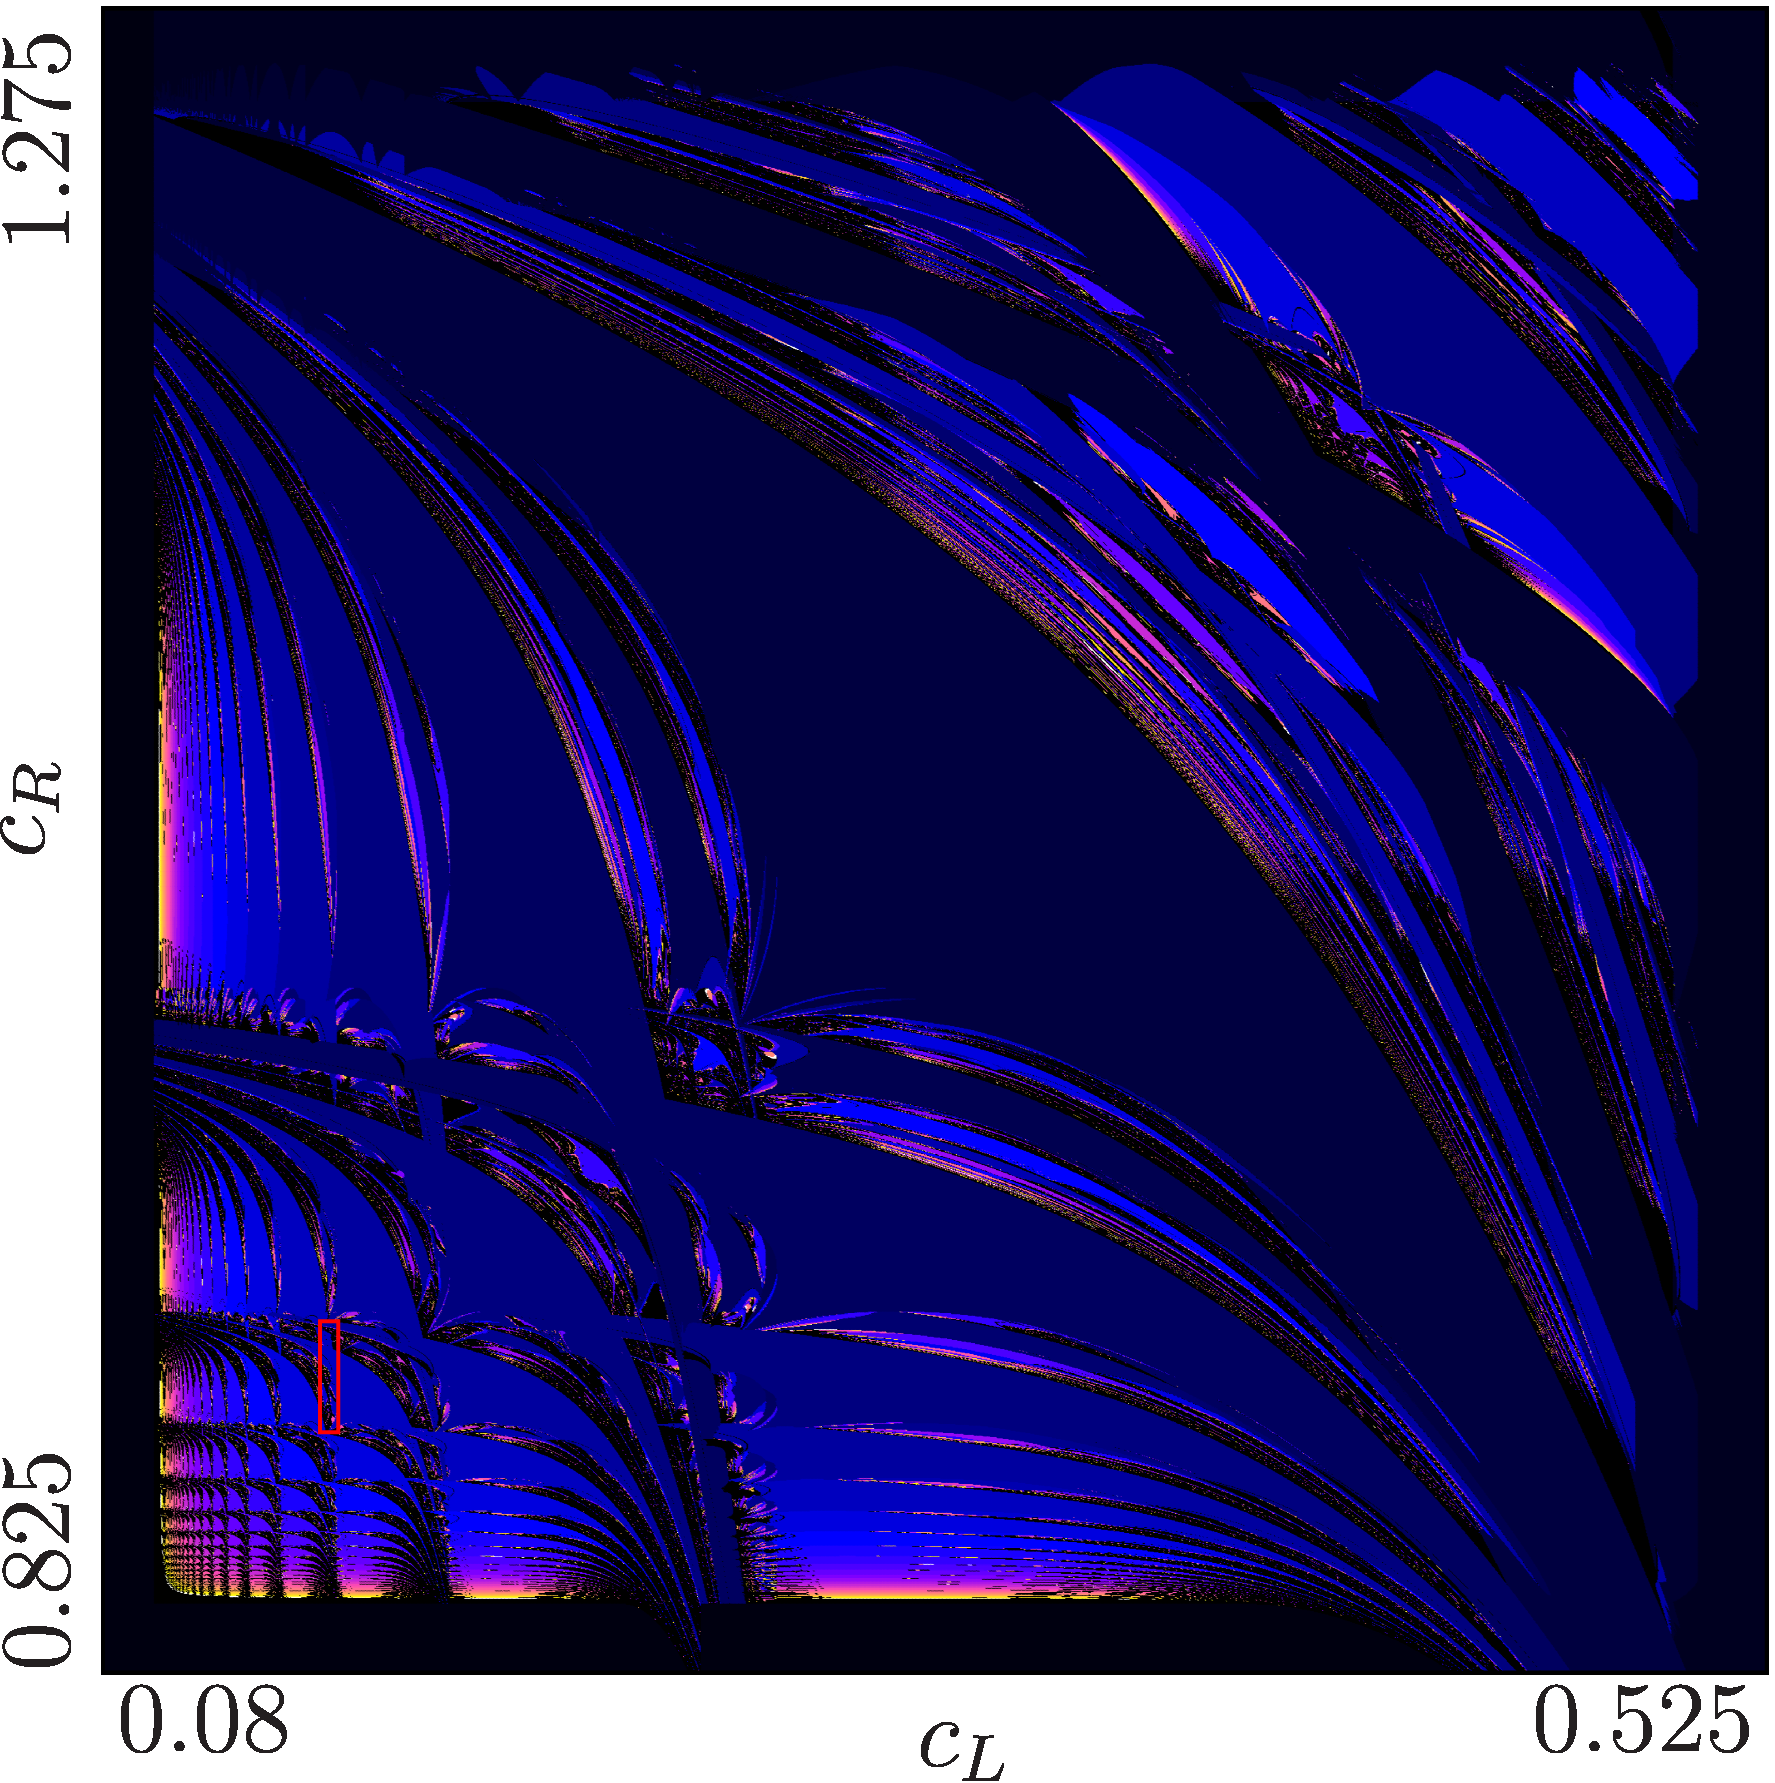
\includegraphics[width=.48 \textwidth]{../Figures/5/5.7a/result.png}
		\label{fig:setup.quad.skew.period.full}
	}
	\subfloat[Zoomed]{
		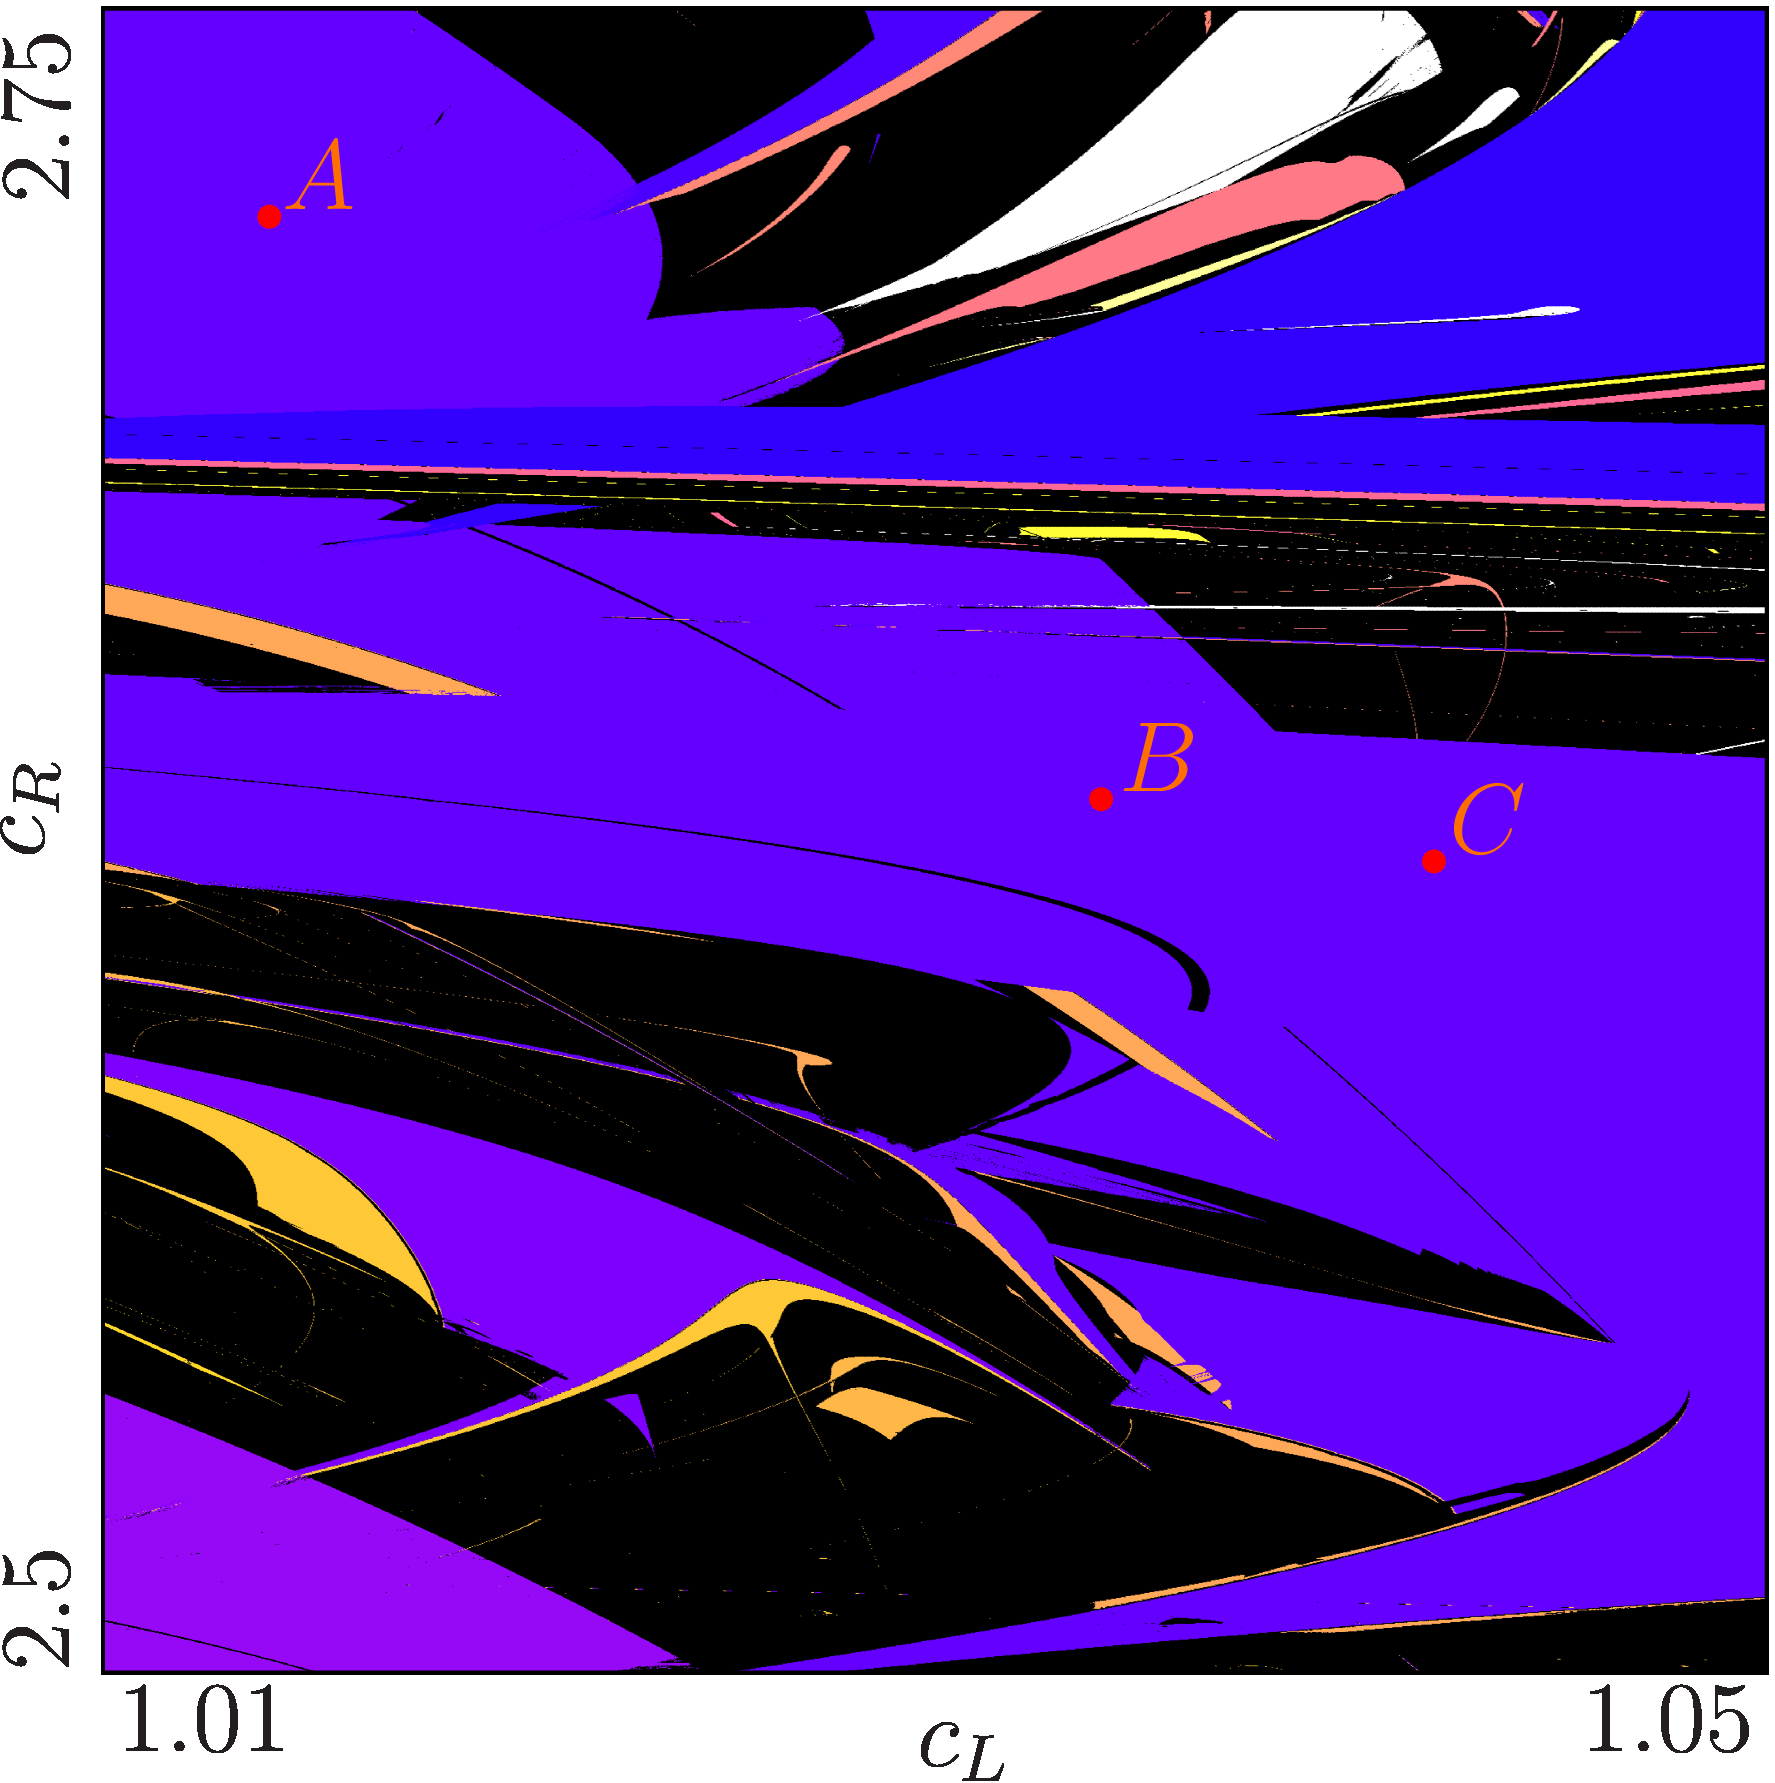
\includegraphics[width=.48 \textwidth]{../Figures/5/5.7b/result.png}
		\label{fig:setup.quad.skew.period.zoomed}
	}
	\caption[2D scans of the periods associated with parameter regions in the piecewise-quadratic model with shifted parabola-shaped branches]{
		2D scans of the periods associated with parameter regions in the piecewise-quadratic model with shifted parabola-shaped branches.
		The parameters $a_L = a_R = 6$, $b_L = -\frac{1}{2}$, and $b_R = -\frac{7}{2}$ are fixed.
		The parameters $c_L$ and $c_R$ are varied in different ranges.
		(a) shows the full structure with the parameters being varied in the ranges $[0.08, 0.525]$ and $[0.825, 1.275]$,
		(b) shows a magnified version with the parameters being varied in the ranges $[1.01, 1.05]$ and $[2.5, 2.75]$.
		These parameter ranges are marked with a red rectangle in (a).
		The points in (b) mark the parameter values for the cobweb diagrams in \Cref{fig:setup.quad.skew.cobwebs}
	}
	\label{fig:setup.quad.skew.period}
\end{figure}

\begin{figure}
	\centering
	\subfloat[$A$]{
		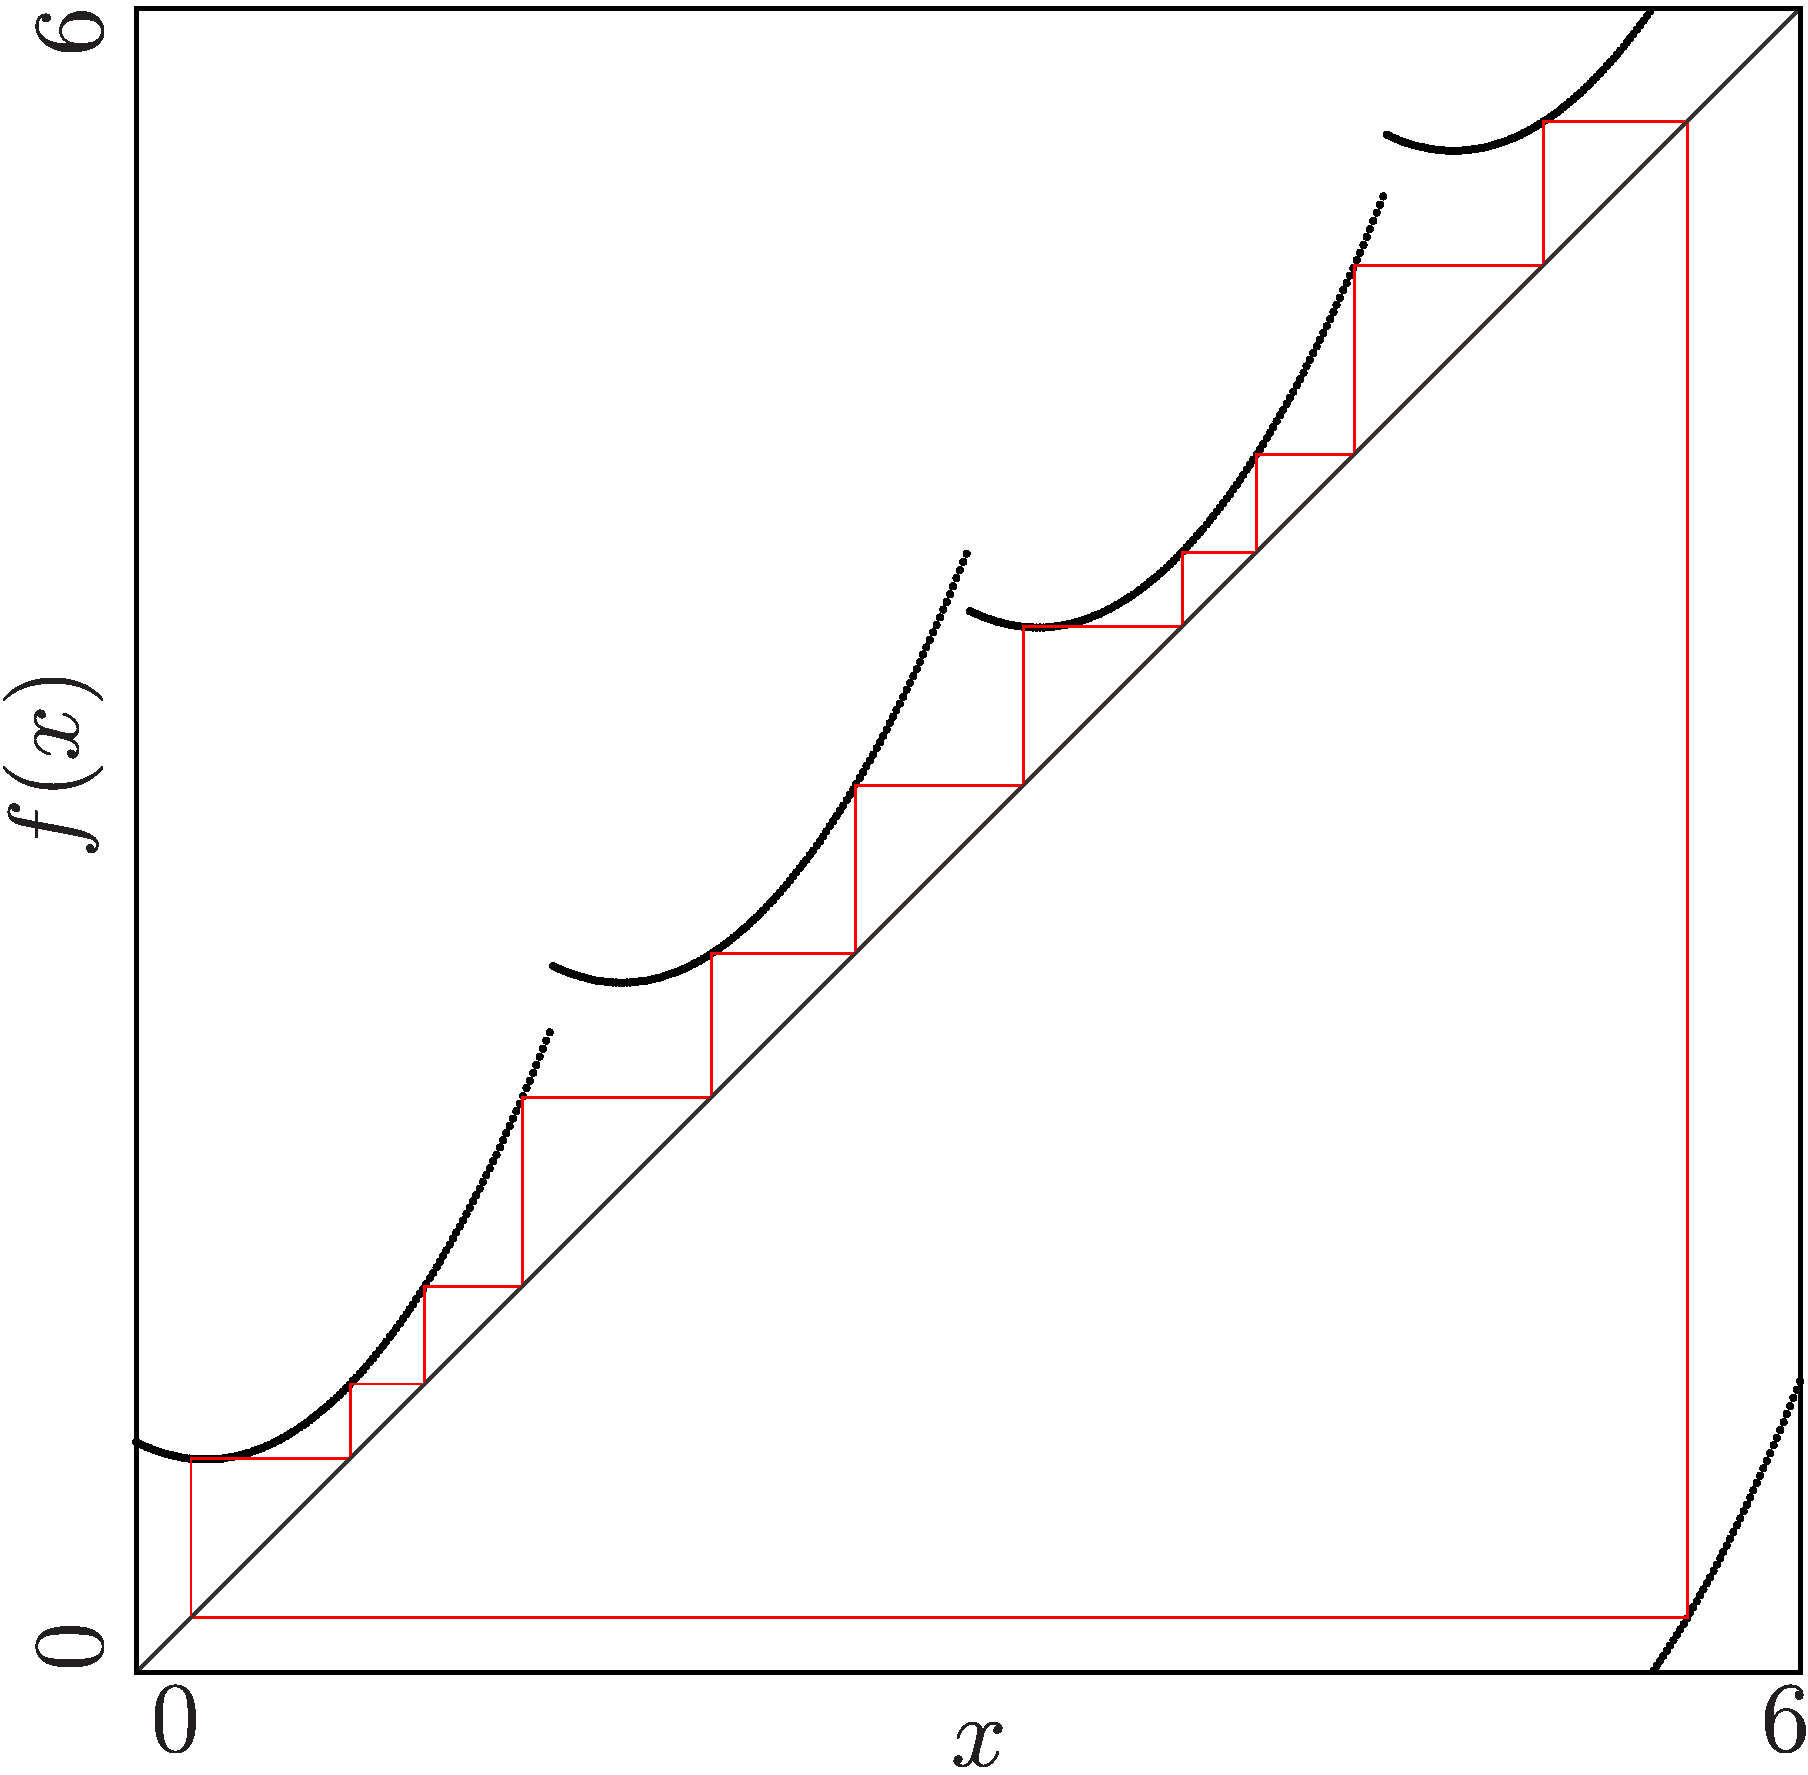
\includegraphics[width=.3 \textwidth]{../Figures/5/5.8a/result.png}
		\label{fig:setup.quad.skew.cobweb.A}
	}
	\subfloat[$B$]{
		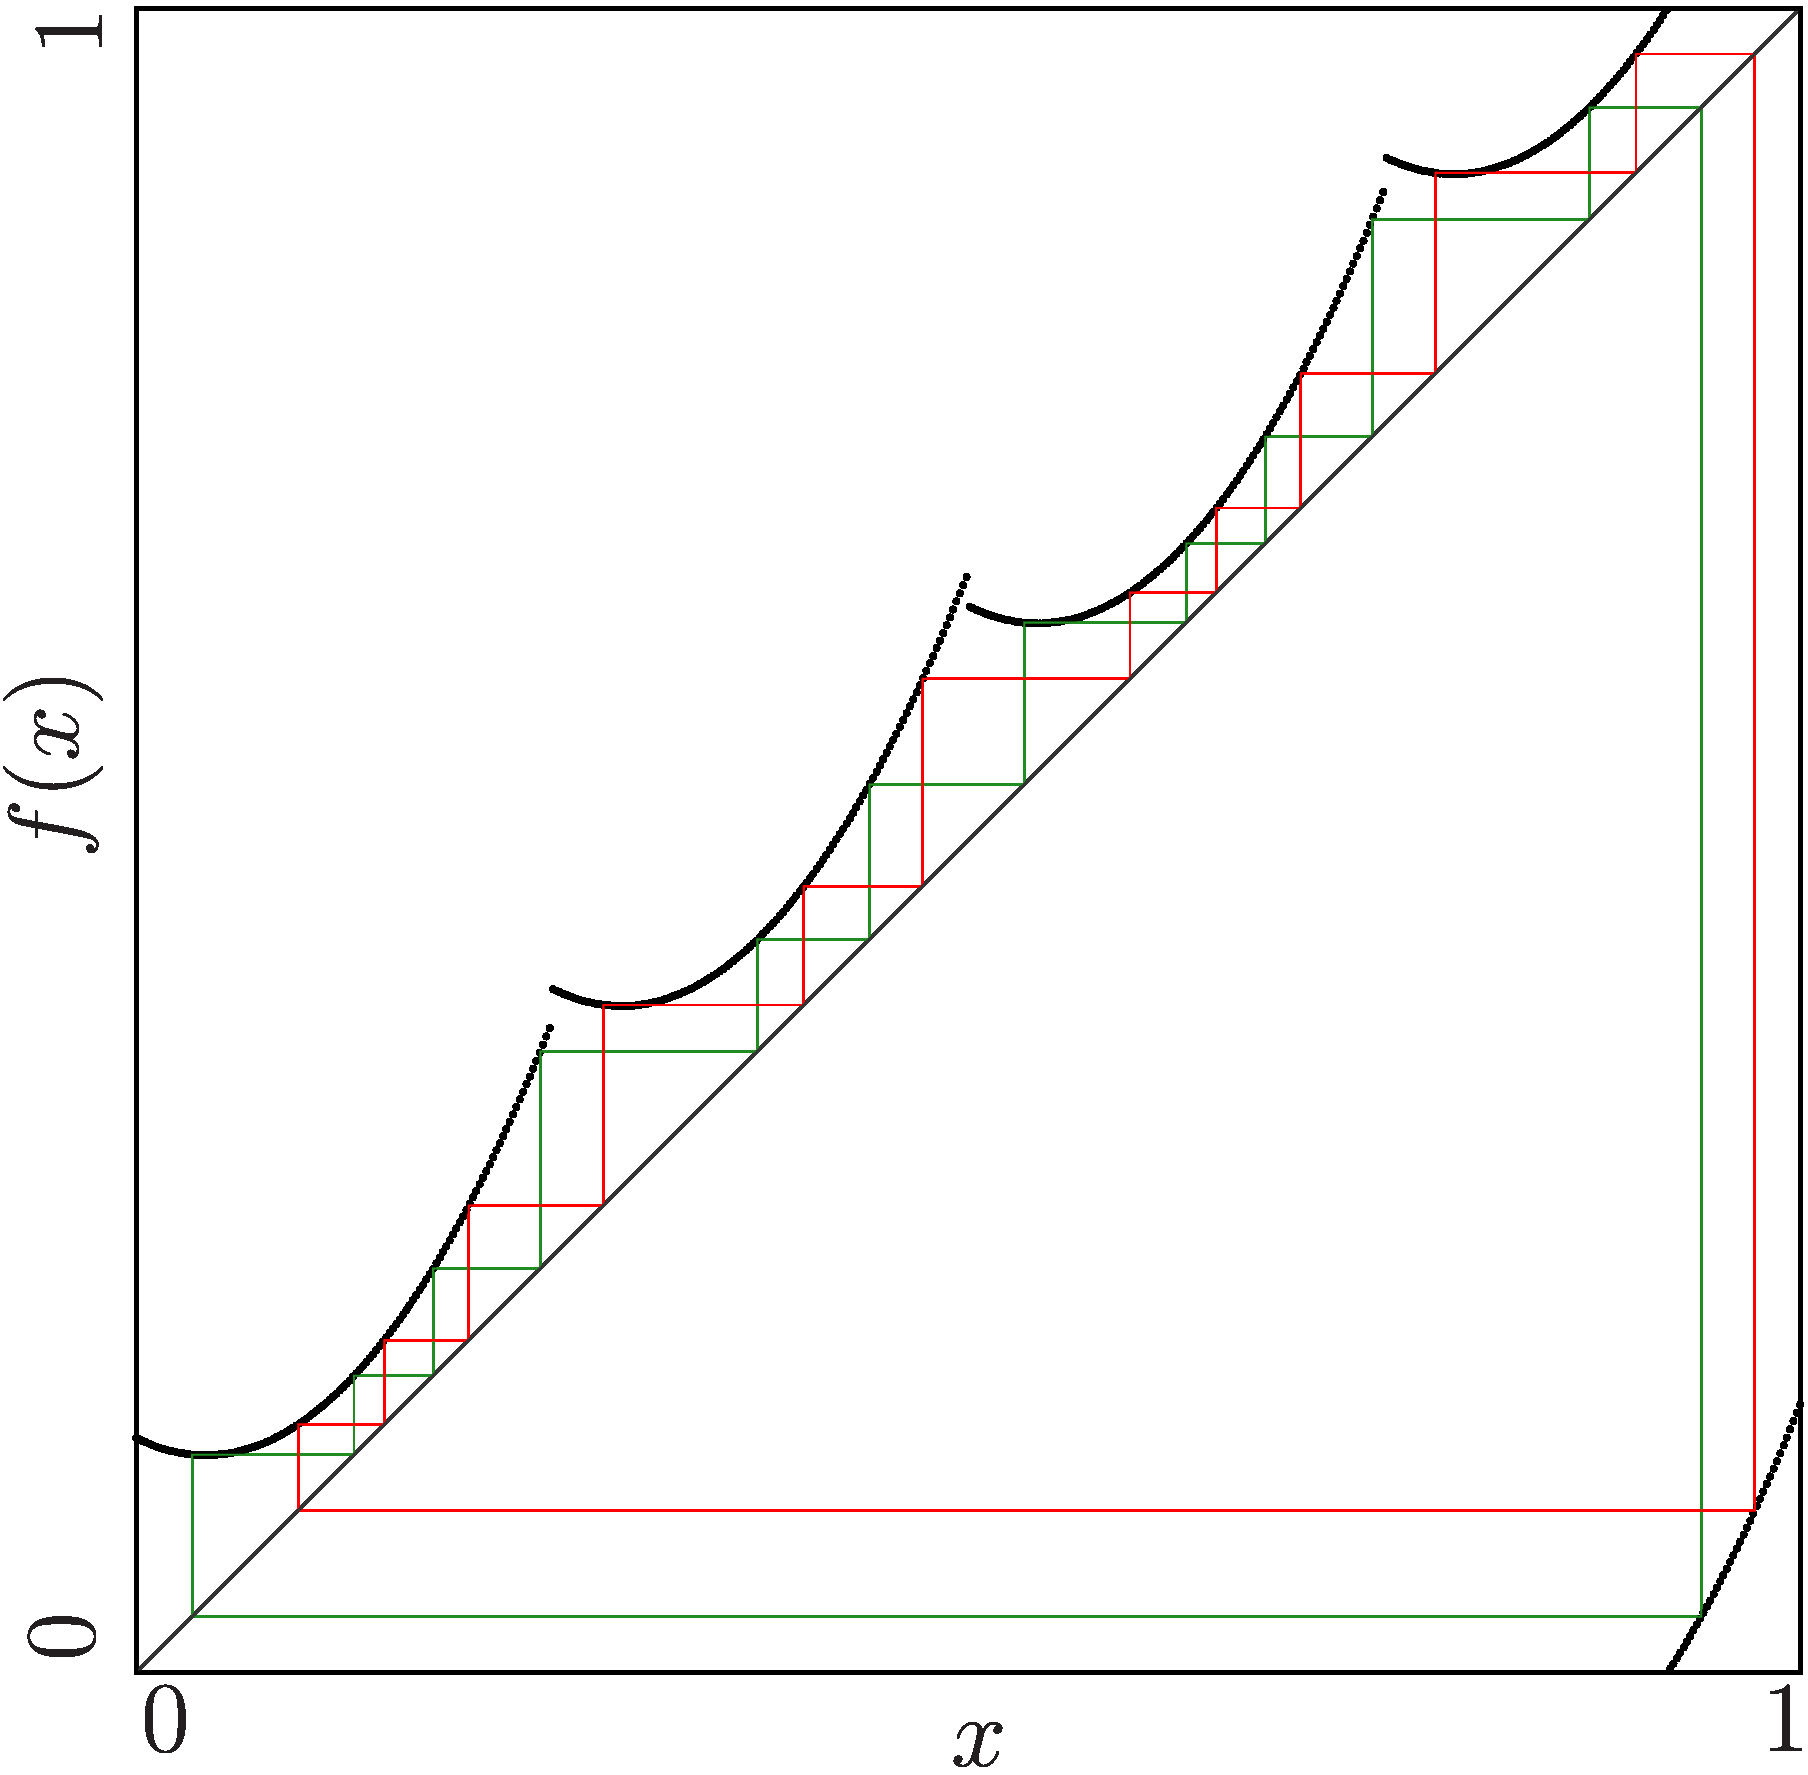
\includegraphics[width=.3 \textwidth]{../Figures/5/5.8b/result.png}
		\label{fig:setup.quad.skew.cobweb.B}
	}
	\subfloat[$C$]{
		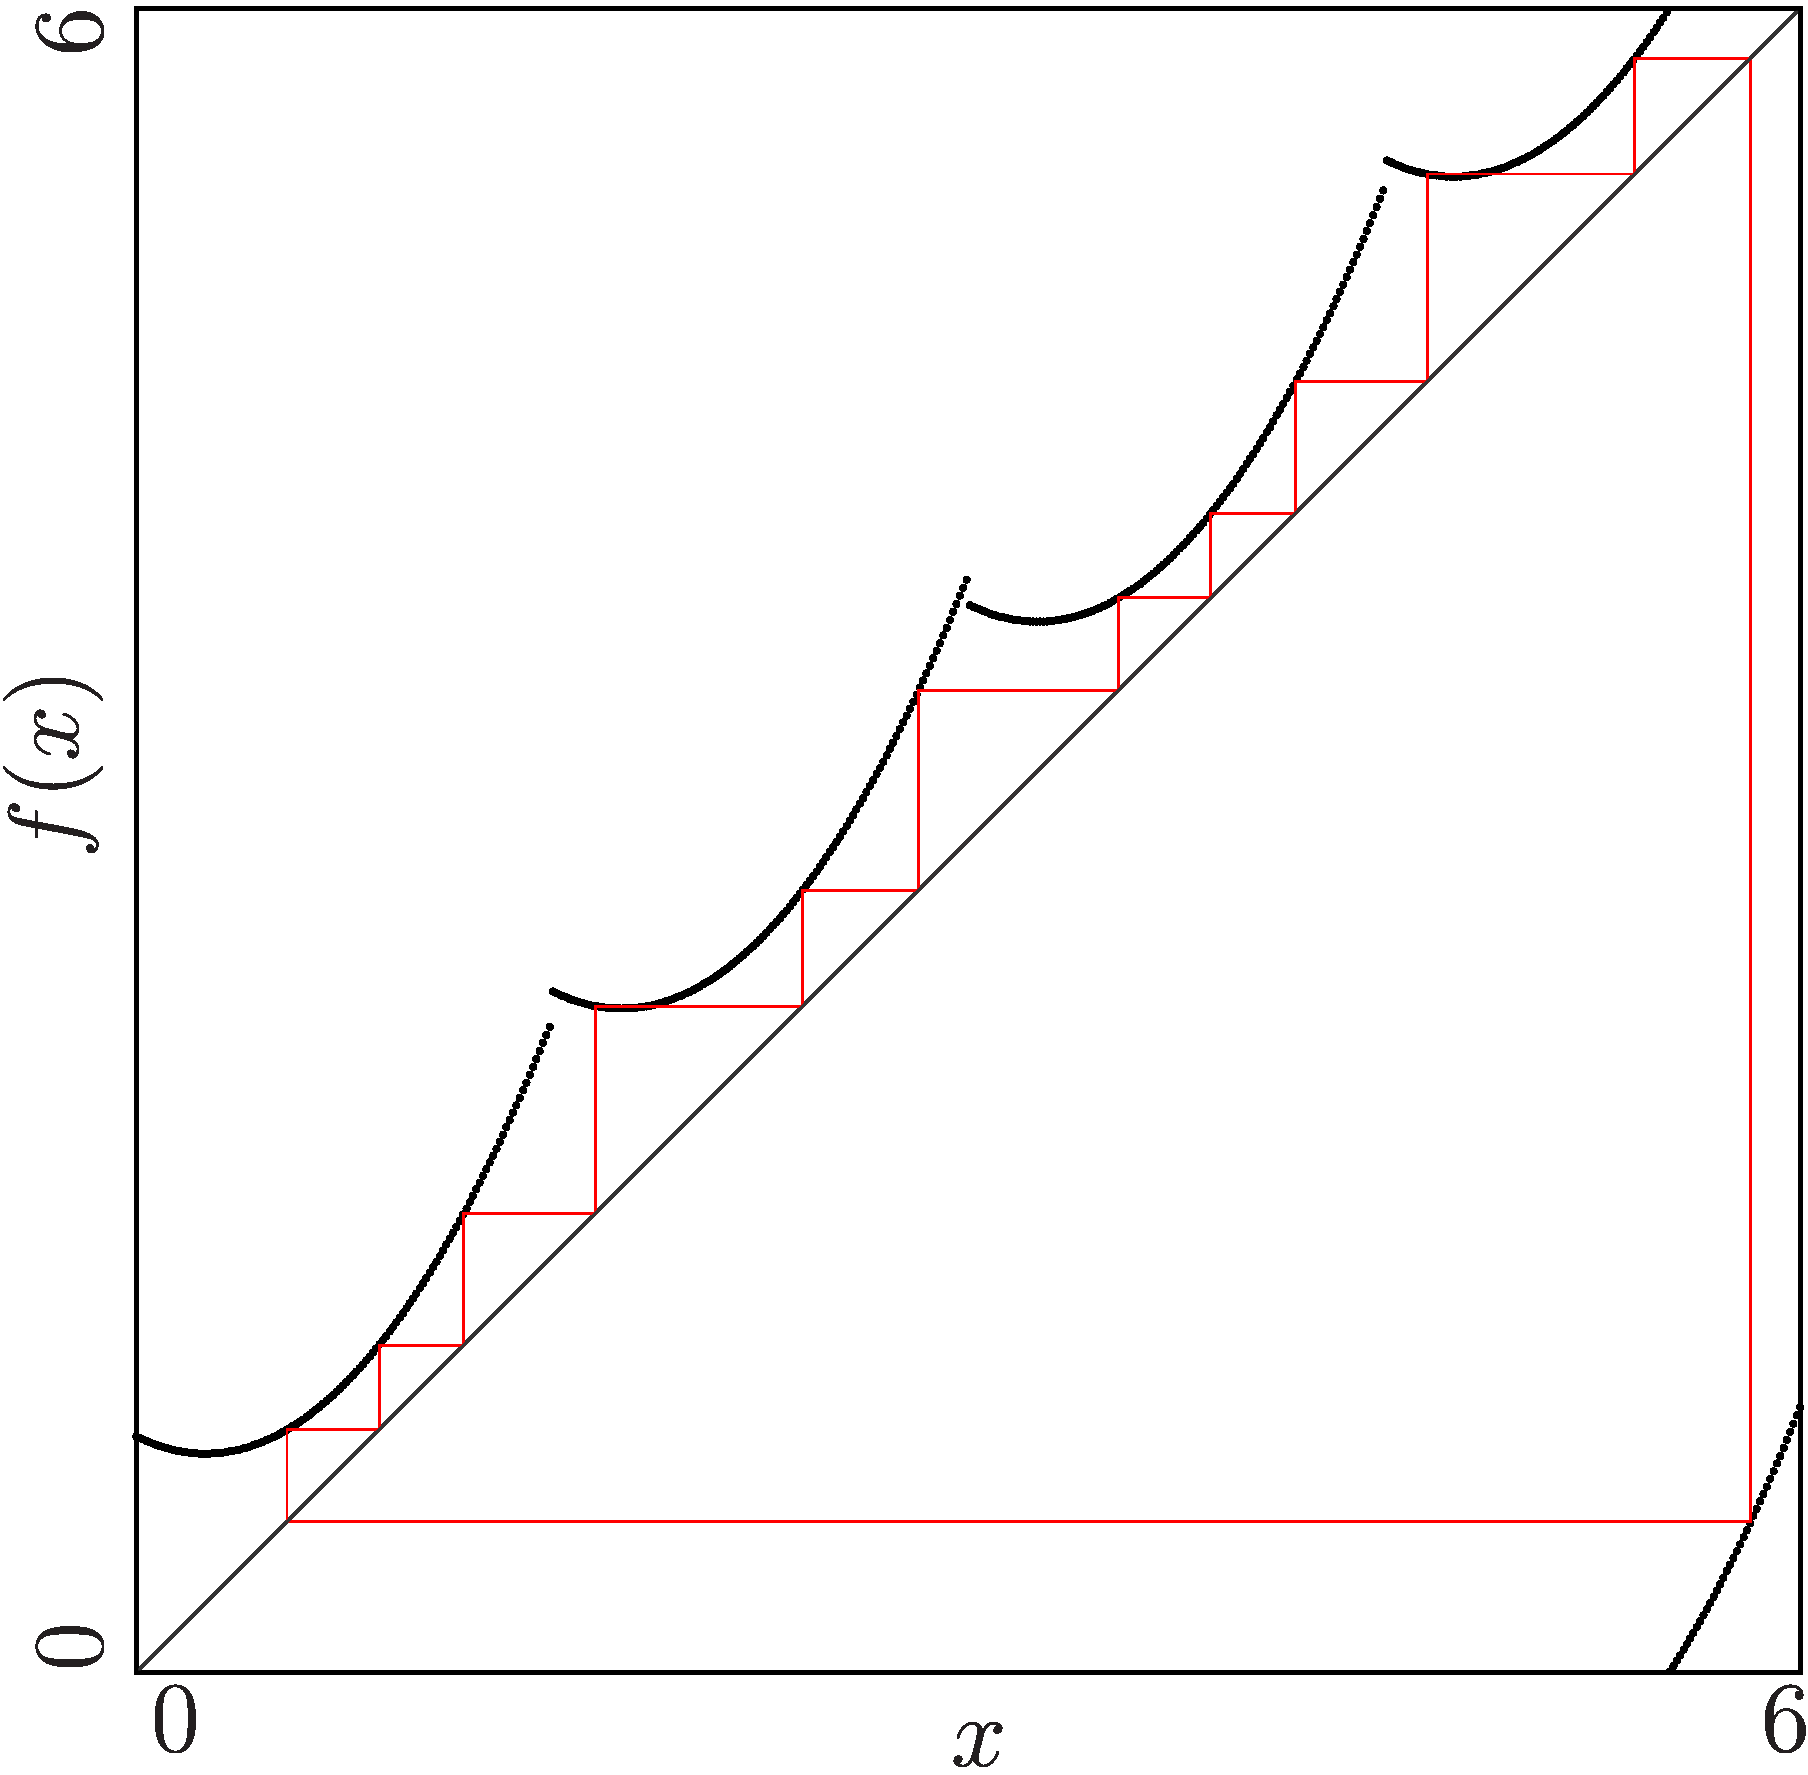
\includegraphics[width=.3 \textwidth]{../Figures/5/5.8c/result.png}
		\label{fig:setup.quad.skew.cobweb.C}
	}
	\caption[Cobweb diagrams of the skewed piecewise quadratic model]{
		Cobweb diagrams at three parameter values of $c_L$ and $c_R$ in the piecewise quadratic model with fixed parameters $a_L = a_R = 6$, $b_L = -\frac{1}{2}$, and $b_R = -\frac{7}{2}$.
		The parameter values are marked in \Cref{fig:setup.quad.even.period.zoomed}.
		(a) shows the cycle $\Cycle{\A^3\B^3\C^3\D^3}$ at point $A$ where $c_L = 0.1385$ and $c_R = 0.925$,
		(b) shows the two coexisting cycles $\Cycle{\A^3\B^3\C^3\D^3}$ (green) and $\Cycle{\A^4\B^2\C^4\D^2}$ (red) at point $C$ where $c_L = 0.141$ and $c_R = 0.911$,
		and (c) shows the cycle $\Cycle{\A^4\B^2\C^4\D^2}$ where $c_L = 0.142$ and $c_R = 0.9095$.
	}
	\label{fig:setup.quad.skew.cobwebs}
\end{figure}

\Cref{fig:setup.quad.skew.cobwebs} shows all the cobweb diagrams of the model at with the parameter values marked in \Cref{fig:setup.quad.skew.period.zoomed}.
The cobweb at point $A$ is shown in \Cref{fig:setup.quad.skew.cobweb.A}.
One can see that it has period 12 and its symbolic sequence is $\A^4\B^2\C^4\D^2$.
The cycle at point $C$ also has period 12.
Its cobweb diagram is shown in \Cref{fig:setup.quad.skew.cobweb.C}, and one can see that its symbolic sequence is $\A^3\B^3\C^3\D^3$.

From point $A$ to point $C$, one point of the cycle on the branch $f_\A$ moved to the branch $f_\B$.
The same thing happened to a point of the cycle on the branch $f_\C$, it moved to the branch $f_\D$.
This is similar to what happens in the original model along a chain of parameter regions with the same period.
And in between both points, there is a parameter region where 2 cycles coexist.
This is shown in \Cref{fig:setup.quad.skew.cobweb.B}, which depicts the cycles at point $C$.
But unfortunately, the coexisting cycles are the same cycles that exist at point $A$ and point $C$, $\Cycle{\A^4\B^2\C^4\D^2}$ and $\Cycle{\A^3\B^3\C^3\D^3}$.
Similarly to the previous experiment, we merely observe two parameter regions with stable cycles overlapping, see \Cref{sec:setup.quad.even}.
